\documentclass[a4paper, 10pt, ]{article}

\usepackage[slovak]{babel}

\usepackage[utf8]{inputenc}
\usepackage[T1]{fontenc}

\usepackage[left=4cm,
			right=4cm,
			top=2.1cm,
			bottom=2.6cm,
			footskip=7.5mm,
			twoside,
			marginparwidth=3.5cm,
			%showframe,
			]{geometry}

\usepackage{graphicx}
\usepackage{xcolor}

% ------------------------------

\usepackage{lmodern}

\usepackage[tt={oldstyle=false,proportional=true,monowidth}]{cfr-lm}

% ------------------------------

\usepackage{amsmath}
\usepackage{amssymb}
\usepackage{amsthm}

\usepackage{booktabs}
\usepackage{multirow}
\usepackage{array}
\usepackage{dcolumn}

\usepackage{natbib}

\usepackage[singlelinecheck=true]{subfig}


% ------------------------------


\usepackage{sectsty}
\allsectionsfont{\sffamily}


\usepackage{titlesec}
\titleformat{\paragraph}[hang]{\sffamily  \bfseries}{}{0pt}{}
\titlespacing*{\paragraph}{0mm}{3mm}{1mm}


\usepackage{fancyhdr}
\fancypagestyle{plain}{%
\fancyhf{} % clear all header and footer fields
\fancyfoot[C]{\sffamily {\bfseries \thepage}\ | {\scriptsize\oznacenieCasti}}
\renewcommand{\headrulewidth}{0pt}
\renewcommand{\footrulewidth}{0pt}}
\pagestyle{plain}


% ------------------------------


\makeatletter

	\def\@seccntformat#1{\protect\makebox[0pt][r]{\csname the#1\endcsname\hspace{5mm}}}

	\def\cleardoublepage{\clearpage\if@twoside \ifodd\c@page\else
	\hbox{}
	\vspace*{\fill}
	\begin{center}
	\phantom{}
	\end{center}
	\vspace{\fill}
	\thispagestyle{empty}
	\newpage
	\if@twocolumn\hbox{}\newpage\fi\fi\fi}

	\newcommand\figcaption{\def\@captype{figure}\caption}
	\newcommand\tabcaption{\def\@captype{table}\caption}

\makeatother


% ------------------------------


\def\naT{\mathsf{T}}

\hyphenpenalty=6000
\tolerance=6000


% ------------------------------


\usepackage[pdfauthor={MT},
			pdftitle={AR},
			pdfsubject={},
			pdfkeywords={},
			linkbordercolor = white,
			%citebordercolor = white,
			breaklinks,
			]{hyperref}


\def\oznacenieCasti{AR05 - LS2019}





\begin{document}





\fontsize{12pt}{22pt}\selectfont

\centerline{\textsf{Adaptívne riadenie} \hfill \textsf{\oznacenieCasti}}

\fontsize{18pt}{22pt}\selectfont





\begin{flushleft}
	\textbf{\textsf{MRAC gradientný}}
\end{flushleft}





\normalsize

\bigskip

\tableofcontents

\bigskip

\vspace{18pt}






\noindent
V prvom rade poznámka k nadpisu: MRAC je skratka z \emph{Model Reference Adaptive Control}, čo znamená Adaptívne riadenie s referenčným modelom. Ide o istú schému priameho adaptívneho riadenia, ktorá pre návrh zákona adaptácie využíva myšlienku o gradiente istej účelovej funkcie, ktorej optimom je vlastne splnenie cieľa riadenia. Slangovo povedané: MRAC („mrak“) gradientný.








\begin{figure}[!b]
\centering

	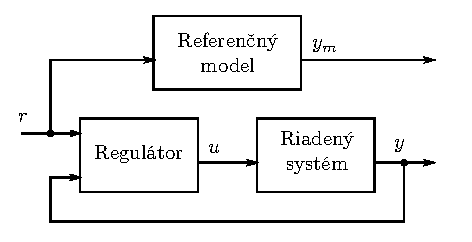
\includegraphics{Obr_RiadSRefModSch_standalone.pdf}

	\caption{Riadenie s referenčným modelom -- principiálna schéma}
	\label{Riadenie s referenčným modelom --- principiálna schéma}

\end{figure}





\section{Riadenie s referenčným modelom}

Pri riadení s~referenčným modelom (\emph{model reference control -- MRC}) sú žiadané vlastnosti uzavretého regulačného obvodu opísané referenčným modelom, čo je jednoducho lineárny, časovo invariantný systém s~prenosovou funkciou $W_m(s)$, ktorého vstupom je referenčná (žiadaná) veličina (hodnota) $r$. Do referenčného modelu sa premietnu požiadavky na výsledný regulačný obvod -- URO. Výstup referenčného modelu $y_m$ sa potom správa práve tak, ako to žiadame od výstupnej (riadenej) veličiny systému.  URO je chápaný ako celok, ktorý vznikne pripojením zákona riadenia (regulátora) k~riadenému systému. Vstupom URO je referenčná veličina $r$~a~výstupom je výstupná veličina systému $y$. Podobným spôsobom sa predpisujú požiadavky pri návrhoch napr. servo-systémov.


Zákon riadenia  je zostavený tak, že prenosová funkcia URO má rovnakú štruktúru (tvar) ako referenčný model. Tým je daná štruktúra (tvar) zákona riadenia. Nie že by štruktúra bola daná jednoznačne, jednoducho, zákon riadenia musí byť taký, že umožní zhodu URO a~referenčného modelu. Otázkou ostáva nastavenie parametrov, ktoré zákon riadenia obsahuje.

V~predchádzajúcom príklade, v ktorom sme sa venovali adaptívnej stabilizácii, má zákon riadenia tvar $u = -k\, x$. Parameter zákona riadenia je $k$. Pri lineárnom regulátore, teda keď je jednoznačné, že parameter $k$ je konštanta, nemení sa v čase, je $k$ určené jednoduchou podmienkou, ktorá však vyžaduje znalosť parametra sústavy. V~prípade riadiaceho systému, kde sa pripúšťa, že $k$ sa môže (a má!) meniť v čase (adaptovať sa) je $k$ v~každom čase určené predpisom v tvare diferenciálnej rovnice.








\begin{figure}[!t]
\centering

	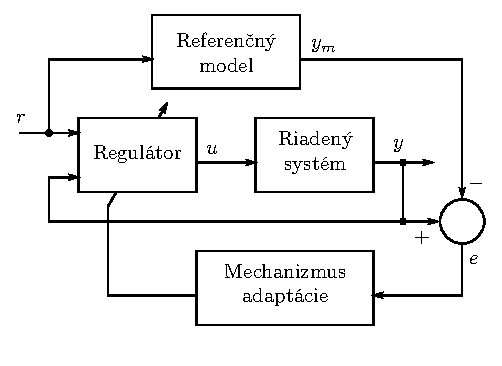
\includegraphics{Obr_AdaptRiadSRefModSch_standalone.pdf}

	\caption{Adaptívne riadenie s referenčným modelom -- principiálna schéma}
	\label{Adaptívne riadenie s referenčným modelom --- principiálna schéma}

\end{figure}







\subsection{MRAC}

Na princípe riadenia s referenčným modelom je založená široká trieda metód adaptívneho riadenia nazývaná \emph{Adaptívne riadenie s~referenčným modelom} čo je prekladom z angličtiny: \emph{Model Reference Adaptive Control -- MRAC}. Niekedy sa zvykne takýto systém riadenia skratkou MRAS -- Model Reference Adaptive System.

Pri adaptívnom riadení s referenčným modelom obsahuje riadiaci systém bežnú spätnoväzbovú slučku, v ktorej sú riadený systém a~regulátor. Ako už bolo uvedené ďalšia spätnoväzbovú slučka v~systéme mení parametre regulátora. Bežná spätnoväzbová slučka sa niekedy nazýva aj vnútorná slučka a~spätnoväzbová slučka pre nastavovanie parametrov regulátora sa nazýva vonkajšia slučka. V~tomto prípade je spätnou väzbou vo vonkajšej slučke rozdiel medzi výstupom riadeného systému a~referenčného modelu, ktorý sa nazýva \emph{adaptačná odchýlka}, označuje sa $e$.

Mechanizmus, ktorý adaptuje parametre regulátora (zákona riadenia) môže byť v adaptívnom riadení s~referenčným modelom získaný dvomi spôsobmi. Použitím gradientnej metódy alebo použitím Lyapunovovej teórie stability. Oba prípady sú predmetom ďalších častí, pričom prvý uvedený je označený ako MRAC -- gradientntný.









\section{MIT algoritmus adaptácie: MRAC gradientný}



Takzvané MIT pravidlo (MIT rule) je pôvodný mechanizmus adaptácie používaný v adaptívnom riadení s~referenčným modelom. Názov vyplýva zo skutočnosti, že bol vyvinutý na MIT (Massachusetts Institute of Technology). Základnú myšlienku vyjadríme v nasledujúcom príklade.

Uvažujme, pre riadenie systému s~výstupom $y$ je použitý regulátor s~jedným nastaviteľným parametrom $\Theta$. Želané správanie uzavretého regulačného obvodu je špecifikované pomocou referenčného modelu, ktorého výstup je veličina $y_m$. Nech $e = y - y_m$ je adaptačná odchýlka. Jednou z možností ako postupovať pri nastavovaní parametra $\Theta$ je meniť ho tak aby sa účelová funkcia v tvare
\begin{equation}
	J(\Theta) = \frac{1}{2} e^2
\end{equation}
minimalizovala. Pre zníženie hodnoty funkcie $J$, je rozumné meniť parameter $\Theta$~proti smeru derivácie $J$~podľa $\Theta$~(gradientu funkcie), teda zmenu parametrov možno vyjadriť v tvare
\begin{equation}
	\frac{\text{d}\Theta}{\text{d}t} = - \alpha \frac{\partial J}{\partial \Theta} = - \alpha e \frac{\partial e}{\partial \Theta}
\end{equation}
kde $\alpha > 0$ je voliteľný parameter pre nastavenie veľkosti zmeny adaptovaného parametra a teda rýchlosti adaptácie, nazýva sa aj \emph{adaptačné zosilnenie}. Toto je princíp slávneho MIT algoritmu adaptácie parametrov regulátora.

Tento algoritmus možno použiť aj keď regulátor obsahuje viac ako jeden parameter. Potom $\Theta$ nie je skalár ale vektor a výraz $\frac{\partial J}{\partial \Theta}$ je skutočne gradientom.

Tiež je možné algoritmus modifikovať použitím inej účelovej funkcie, pričom princíp ostáva zachovaný.

Parciálna derivácia $\frac{\partial e}{\partial \Theta}$ sa nazýva \emph{citlivostná funkcia}, hovorí o tom ako veľmi je adaptačná odchýlka $e$~ovplyvnená zmenou parametrov regulátora. Túto funkciu je možné vyjadriť pri predpoklade, že zmeny parametrov regulátora sú o veľa pomalšie ako zmeny všetkých ostatných veličín v~systéme. Potom parametre regulátora môžme považovať za nezávislé od času. V~ďalšom sa ukáže, že citlivostné funkcie často (nie vždy ako ukazuje nasledujúca časť) obsahujú parametre sústavy a teda neznáme parametre. Preto ich nie je možné priamo použiť a je potrebné nájsť ich vhodnú aproximáciu, takú, ktorá neobsahuje neznáme parametre.






\subsection{Adaptácia dopredného zosilnenia}

Uvažujme riadený systém daný prenosovou funkciou v~tvare
\begin{equation}
	\frac{y(s)}{u(s)} = \frac{k}{s + 1}
\end{equation}
kde $k$ je neznámy parameter, ale znamienko parametra $k$ je známe. Úlohou je nájsť dopredný regulátor, ktorý spolu s prenosovou funkciou bude tvoriť systém špecifikovaný referenčným modelom. Referenčný model je definovaný v tvare prenosovej funkcie
\begin{equation} \label{pfRefModelu}
	\frac{y_m(s)}{r(s)} = \frac{k_m}{s + 1}
\end{equation}

Uvažujme zákon riadenia v tvare
\begin{equation}
	u = \Theta r
\end{equation}
kde $u$~je akčný zásah (vstup riadeného systému) a~$r$~je žiadaná hodnota. Tento zákon riadenia umožní, že prenosová funkcia zo žiadanej hodnoty $r$~na výstupnú veličinu $y$~je v~tvare
\begin{equation} \label{pfURO}
	\frac{y(s)}{r(s)} = \frac{k \Theta}{s + 1}
\end{equation}
Prenosová funkcia \eqref{pfURO} sa zhoduje s prenosovou funkciou referenčného modelu \eqref{pfRefModelu} ak
\begin{equation} \label{LePodmZhody}
	\Theta^\star = \frac{k_m}{k}
\end{equation}
kde parameter regulátora je označený symbolom $^\star$ pretože je to ideálna hodnota, pri ktorej je cieľ riadenia splnený. Táto hodnota však nie je známa, pretože $k$ nie je známe. Veľmi dôležité však je, že sme tým ukázali existenciu takej hodnoty. Ak by ani teoreticky neexistovala ideálna hodnota parametra regulátora, ktorú adaptujeme, samotná adaptácia by nemala zmysel. Rovnica \eqref{LePodmZhody} sa nazýva podmienka zhody a pri návrhu adaptívneho riadenia je vždy dôležité ukázať, že podmienky zhody existujú a~že majú riešenie.

Pre návrh zákona adaptácie teraz použijeme MIT algoritmus. Adaptačná odchýlka je
\begin{subequations}
	\begin{align}
		e &= y - y_m \\
		e &= \frac{k \Theta}{s + 1} r - y_m
	\end{align}
\end{subequations}
Pretože $\Theta$ považujeme za nezávislú od času, môžme písať
\begin{equation} \label{parcDerBezAprox}
	\frac{\partial e}{\partial \Theta}
	=
	\frac{k}{s + 1} r
\end{equation}
čo je citlivostná funkcia potrebná, ako už vieme, v zákone adaptácie podľa MIT algoritmu. Obsahuje však neznáme $k$. Ak poznáme znamienko $k$ môže byť toto zosilnenie absorbované do adaptačného zosilnenia $\alpha$. Hodnota $\alpha$ je ľubovolná, preto nie je potrebné poznať presnú hodnotu $k$, len jeho znamienko, aby bolo možné správne zvoliť znamienko konštanty $\alpha$ a zabezpečiť záporné výsledné znamienko v zákone adaptácie. Predpokladali sme, že znamienko $k$ je známe. Preto je možné citlivostnú funkciu použiť v zákone adaptácie tak ako je, okrem zosilnenia $k$. Nie je potrebná žiadna aproximácia ako v iných prípadoch, napríklad v príklade v nasledujúcej časti.

Zákon adaptácie potom je
\begin{align}
	 	s \Theta =  - \alpha e \frac{\partial e}{\partial \Theta}
\end{align}
kde $s$ predstavuje operátor derivácie podľa času. Po dosadení \eqref{parcDerBezAprox}:
\begin{align}
 	s \Theta =  - \alpha k e \frac{1}{s + 1} r = - \alpha  e y_m
\end{align}

Keďže máme predpis pre zmenu adaptovaného parametra, zákon adaptácie, stačí už len integrovať výstup zákona adaptácie a získame tak signál adaptovaného parametra zákona riadenia.

Všimnime si, že v tomto bode na základe uvedeného nemôžme urobiť žiadne závery o stabilite celého adaptívneho systému.

Prípad, keď je potrebné aproximovať citlivostnú funkciu, pretože obsahuje viac neznámych parametrov riadeného systému je opísaný, spolu s ďalšími detailmi, v~nasledujúcej časti.







\subsection{Systém 2. rádu s astatizmom -- príklad}


Uvažujme riadený systém daný prenosovou funkciou v~tvare
\begin{equation} \label{sustavaSoblast}
	\frac{y(s)}{u(s)} = \frac{b_0}{s^2 + a_1 s}
\end{equation}
kde $y(s)$ je obraz výstupného signálu, $u(s)$ je obraz vstupného signálu a $a_1$, $b_0$ sú reálne konštanty -- neznáme parametre sústavy.
V časovej oblasti je modelom sústavy diferenciálna rovnica v tvare
\begin{equation} \label{DRsustavyToblast}
	\ddot{y}(t) + a_1 \dot{y}(t) = b_0 u(t)
\end{equation}
Ide o sústavu druhého rádu s astatizmom. Preto je vhodné použiť pre jej riadenie PD (proporcionálno-derivačný) zákon riadenia v tvare
\begin{equation} \label{PDzakRiadSobl}
	u(s) = \Theta_1 \left(r(s)-y(s)\right) - \Theta_2 s y(s)
\end{equation}
kde $r$ je žiadaná hodnota.
Zákon riadenia \eqref{PDzakRiadSobl} vznikne úpravou štandardného PD regulátora v tvare
\begin{equation} \label{standardPDregSobl}
	u(s) = \left(\Theta_1 + \Theta_2 s\right) e_r(s)
\end{equation}
kde $e_r = r-y$ je regulačná odchýlka, pričom sa predpokladá, že $r(t) = \text{konšt.}$ a teda $\dot{r}(t) = 0$. V časovej oblasti možno napísať štandardný PD regulátor \eqref{standardPDregSobl} v~tvare
\begin{equation}
	u(t) = \Theta_1 \left( r(t) - y(t) \right) + \Theta_2 \left( \dot{r}(t) - \dot{y}(t) \right)
\end{equation}
a upravený PD zákon riadenia \eqref{PDzakRiadSobl} má v časovej oblasti tvar
\begin{equation}
	u(t) = \Theta_1 \left( r(t) - y(t) \right) - \Theta_2  \dot{y}(t)
\end{equation}




Dosadením \eqref{PDzakRiadSobl} do \eqref{sustavaSoblast} získame prenosovú funkciu uzavretého regulačného obvodu (URO) v tvare
\begin{equation} \label{uvGradUROSoblast}
	\frac{y(s)}{r(s)} = \frac{b_0 \Theta_1}{s^2 + \left(a_1 + b_0 \Theta_2 \right) s + b_0 \Theta_1}
\end{equation}

Referenčný model nech je definovaný takto
\begin{equation} \label{uvGradRMSoblast}
	\frac{y_m(s)}{r(s)}  =  \frac{b_{0m} }{s^2 + a_{1m} s + a_{0m}}
\end{equation}
kde $b_{0m}=a_{0m}$ a $a_{1m}$ sú konštanty. Je zrejmé, že ideálne parametre regulátora sú
\begin{align}
	\Theta_1^\star &= \frac{a_{0m}}{b_0} \\
	\Theta_2^\star &= \frac{a_{1m} - a_1}{b_0}
\end{align}
Pri ideálnych parametroch je adaptačná odchýlka $e$~nulová
\begin{equation} \label{gradDefAdaptE}
	e = y - y_m
\end{equation}

Definujme účelovú funkciu vektora parametrov  $\Theta = \begin{bmatrix} \Theta_1 & \Theta_2  \end{bmatrix}^{T}$ v tvare
\begin{equation}
	J(\Theta) = \frac{1}{2}e^2(\Theta,t)
\end{equation}
Pri ideálnych parametroch $\Theta^\star$ je adaptačná odchýlka $e$ nulová a účelová funkcia $J(\Theta)$ nadobúda munimum. Preto navrhnime zákon adaptácie parametrov $\Theta$ tak aby sme sa pri ich zmene (adaptácii) pohybovali proti smeru gradientu (vzhľadom na parametre $\Theta$) kvadratickej účelovej funkcie a teda zmenšovali hodnotu účelovej funkcie pretože sa tak približujeme k jej extrému -- minimu. Potom aj adaptačná odchýlka $e$ sa bude zmenšovať a výstupná veličina $y$ bude sledovať priebeh veličiny $y_m$, čo je cieľom riadenia. Zákon adaptácie nech má tvar
\begin{equation}
	\dot\Theta
	=
	- \alpha
	\frac{\partial J}{\partial \Theta}
\end{equation}
kde $\frac{\partial J}{\partial\Theta}$ je gradient $J$ vzhľadom na parametre $\Theta$ a určuje kladný smer, preto je použité znamienko mínus, čím dostávame smer \uv{proti gradientu} a $\alpha$ je ľubovolná kladná konštanta, ktorá umožňuje nastaviť \uv{krok} pohybu, presnejšie rýchlosť pohybu proti smeru gradientu. Parameter $\alpha$ sa v adaptívnom riadení nazýva \emph{rýchlosť adaptácie} alebo aj \emph{adaptačné zosilnenie}.




Vyjadrime $\frac{\partial J}{\partial\Theta}$ v tvare
\begin{equation}
	\frac{\partial J}{\partial \Theta}
	= \frac{\partial}{\partial \Theta} \left( \frac{1}{2}e^2(\Theta,t) \right)
	= \frac{1}{2} 2 e(\Theta,t) \frac{\partial e(\Theta,t)}{\partial \Theta}
	= e \frac{\partial e}{\partial \Theta}
\end{equation}
potom zákon adaptácie je v tvare
\begin{equation}
	\dot\Theta = - \alpha e \frac{\partial e}{\partial \Theta}
\end{equation}

Rovnicu \eqref{gradDefAdaptE} možno písať v tvare
\begin{equation} \label{gradAdaptE}
\begin{split}
	e &= \frac{b_0 \Theta_1}{s^2 + \left(a_1 + b_0 \Theta_2 \right) s + b_0 \Theta_1} r - y_m \\
	&= b_0 \Theta_1
	\left(
		s^2 + \left(a_1 + b_0 \Theta_2 \right) s + b_0 \Theta_1
	\right)^{-1}
	r - y_m
	\end{split}
\end{equation}

Parciálna derivácia rovnice \eqref{gradAdaptE} podľa prvého parametra $\Theta_1$ je
\begin{equation} \label{citl1Neaprox}
\begin{split}
	\frac{\partial e}{\partial \Theta_1}
	&=
	\left(
		\left(
			b_0
		\right)
		\left(
			s^2 + \left( a_1 + b_0 \Theta_2 \right) s + b_0 \Theta_1
		\right)^{-1}
	\right.
	\\ & -
	\left.
		\left(
			b_0 \Theta_1
		\right)
			\left(
			s^2 + \left(a_1 + b_0 \Theta_2 \right) s + b_0 \Theta_1
			\right)^{-2}
		b_0
		\right)
	r
	\\ & =
	\left(
		b_0
		\left(
			s^2 + \left( a_1 + b_0 \Theta_2 \right) s + b_0 \Theta_1
		\right)^{-1}
	\right.
	\\ & \cdot
	\left.
		\left(
		1
		-
			b_0 \Theta_1
		\left(
			s^2 + \left(a_1 + b_0 \Theta_2 \right) s + b_0 \Theta_1
			\right)^{-1}
		\right)
	\right)
	r
	\\& =
		b_0
		\left(
			s^2 + \left( a_1 + b_0 \Theta_2 \right) s + b_0 \Theta_1
		\right)^{-1}
	\left(
		r
		-
		y
	\right)
	\end{split}
\end{equation}
a parciálna derivácia rovnice \eqref{gradAdaptE} podľa druhého parametra $\Theta_2$ je
\begin{equation} \label{citl2Neaprox}
\begin{split}
	\frac{\partial e}{\partial {\Theta_2}}
	 & =
	\left(
		b_0 \Theta_1
		(-1)
		\left(
			s^2 + \left( a_1 + b_0 \Theta_2 \right) s + b_0 \Theta_1
		\right)^{-2}
		\left(
			b_0 s
		\right)
	\right)
	r
	\\ & =
	-
	\left(
		b_0 s
	\right)
	\left(
		s^2 + \left( a_1 + b_0 \Theta_2 \right) s + b_0 \Theta_1
		\right)^{-1}
		y
	\end{split}
\end{equation}







Citlivostné funkcie \eqref{citl1Neaprox} a \eqref{citl2Neaprox} obsahujú neznáme parametre sústavy a tiež nateraz neznáme parametre regulátora a preto ich nie je možné použiť. Všimnime si, že ak by mali parametre regulátora práve ideálnu hodnotu, teda ${\Theta}_1 = {\Theta}_1^\star$ a ${\Theta}_2 = {\Theta}_2^\star$ potom platí
\begin{equation}
	s^2 + \left( a_1 + b_0 \Theta_2 \right) s + b_0 \Theta_1 = s^2 + a_{1m} s + a_{0m}
\end{equation}
A ďalej, ak poznáme znamienko konštanty $b_0$ môže byť toto zosilnenie absorbované do adaptačného zosilnenia $\alpha$. Hodnota $\alpha$ je ľubovolná, preto nie je potrebné poznať presnú hodnotu $b_0$, len jeho znamienko, aby bolo možné správne zvoliť znamienko konštanty $\alpha$ a zabezpečiť záporné výsledné znamienko v zákone adaptácie.  Uvážením uvedeného môžeme citlivostné funkcie aproximovať nasledovne
\begin{equation} \label{citl1Aprox}
	\frac{\partial e}{\partial \Theta_1} = \frac{1}{ \left( s^2 + a_{1m} s + a_{0m} \right) } \left( r - y \right)
\end{equation}
\begin{equation} \label{citl2Aprox}
	\frac{\partial e}{\partial \Theta_2} = \frac{-s} { \left( s^2 + a_{1m} s + a_{0m} \right) } \,	y
\end{equation}

Zákony adaptácie pre jednotlivé parametre sú potom v~tvare
\begin{align}
	\Theta_1 s &= - \alpha_1 \left( \frac{1}{ \left( s^2 + a_{1m} s + a_{0m} \right) } \left( r - y \right) \right) \, e \\
	\Theta_2 s &= - \alpha_2 \left( \frac{-s}{ \left( s^2 + a_{1m} s + a_{0m} \right)} \, y \right) \, e
\end{align}
kde sme zaviedli samostatné adaptačné zosilnenia $\alpha_1$ a $\alpha_2$ pre oba zákony adaptácie, čo umožní ich lepšie naladenie.








\section{Cvičenie piate}
\label{cvicpiate}



\begin{enumerate}

	\item  Pri návrhu autopilota pre kormidlovanie nákladnej lode sa používa zjednodušený model lode tzv. Nomotov (K. Nomoto -- vedec, ktorý sa zaoberal návrhom autopilota pre lode) model, ktorý má tvar prenosovej funkcie:
	\begin{equation} \label{NomotoTF}
		\varphi(s) = \frac{\frac{K}{\tau_1}}{s^2 + \frac{1}{\tau_1}s} \, \delta(s)
	\end{equation}
	kde $\varphi(s)$ je uhol natočenia lode v radiánoch (azimut, kurz lode), $\delta$ je uhol vychýlenia kormidla (riadiaca plocha väčšinou v zadnej časti lode ponorená vo vode) v radiánoch. Parametre v prenosovej funkcii \eqref{NomotoTF} sú definované nasledovne
	\begin{align}
		K &= K_0 \frac{v}{L} \\
		\tau_1 &= \tau_{10} \frac{L}{v}
	\end{align}
	kde $v$ je rýchlosť lode v smere danom uhlom $\varphi(s)$ v~metroch za sekundu, $L$ je dĺžka lode v metroch a~$K_0$, $\tau_{10}$ sú konštanty závislé na veľkom množstve faktorov (typ lode atď.) Uvažujme nákladnú loď danú parametrami v Tabuľke~\ref{Parametre lode}.

	\begin{center}
		\catcode`\-=12
		\tabcaption{Parametre lode}
		\label{Parametre lode}
		\begin{tabular}{ c l }
			\toprule
			Parameter & Hodnota \\
			\midrule
			$L$         & $161$ m \\
			$K_0$       &  $-3,86$ \\
			$\tau_{10}$ & $5,66$ \\
			$v$         &  $5$ m s$^{-1}$ \\
			\bottomrule
		\end{tabular}
	\end{center}



	\begin{itemize}
		\item Zostavte simulačný model lode v simulinku.
	\end{itemize}

	\item Požiadavky na dynamiku kormidlovania nákladnej lode nech sú definované referenčným modelom v~tvare prenosovej funkcie:
	\begin{equation}
		\frac{y_m(s)}{r(s)} = \frac{0,0025 }{s^2 + 0,1 s + 0,0025}
	\end{equation}
	kde $r$ je referenčný kurz (rozkaz kapitána) a $y_m$ je požadovaná reakcia lode (priebeh zmeny kurzu).

	\begin{itemize}
		\item Navrhnite adaptívne riadenie s referenčným modelom pre kormidlovanie lode (adaptívny autopilot), pričom zákon adaptácie je založený na gradientnom prístupe a MIT pravidle.

		\item Použite obdĺžnikový referenčný signál $r$. V~jednej perióde rovnomerne rozložené skokové zmeny na úrovne: $5^\circ,0^\circ,-5^\circ,0^\circ$ (Prepočítať na \textbf{radiány}). Dĺžka periódy 1000 sekúnd. Priebeh referenčného signálu je na Obr.~\ref{Referenčný sigál $r$}. Vzorové výsledky simulácie sú na Obr.~\ref{Vzorové výsledky simulácie pre cvičenie druhé}.
	\end{itemize}


	\item Zmeňte rýchlosť lode na $v=4$ [m/s] a $v=6$ [m/s], pričom riadiaci systém ponechajte rovnaký aký ste navrhli pre $v=5$ [m/s]. Pozorujte, či je adaptívny autopilot schopný prispôsobiť sa zmenám. Bonus: vysvetlite pozorované!

\end{enumerate}





\begin{figure}[t]
	\centering

	\subfloat[Referenčný sigál $r$]{%
		\label{Referenčný sigál $r$}
		\makebox[\textwidth][c]{%
		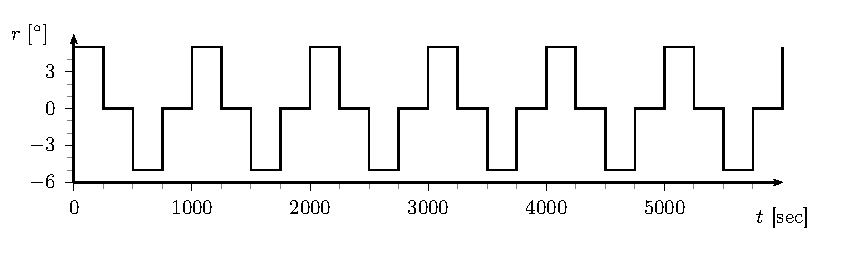
\includegraphics{Obr_cv2Vzor_a.pdf}
		}
	}

	\vspace{-15mm}

	\subfloat[Výstup riadeného systému $y$ a výstup referenčného modelu $y_m$]{%
		\label{Výstup riadeného systému $y$ a výstup referenčného modelu $y_m$}
		\makebox[\textwidth][c]{%
		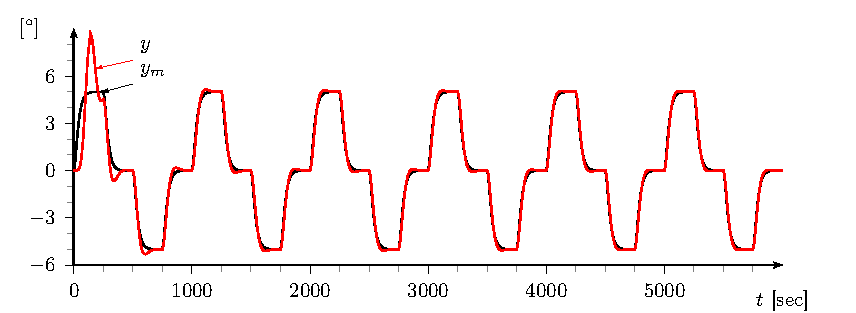
\includegraphics{Obr_cv2Vzor_b.pdf}
		}
	}

	\vspace{-10mm}

	\subfloat[Adaptačná odchýlka $e$]{%
		\label{Adaptačná odchýlka $e$}
		\makebox[\textwidth][c]{%
		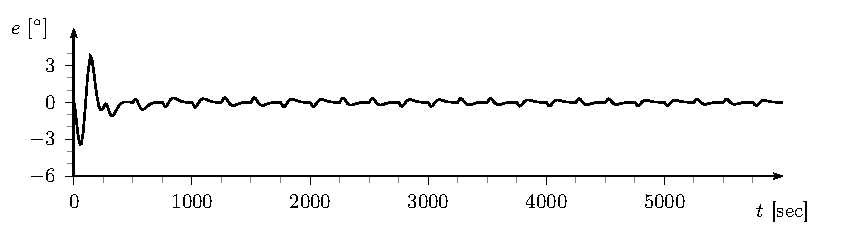
\includegraphics{Obr_cv2Vzor_c.pdf}
		}
}
	\caption{Vzorové výsledky simulácie pre cvičenie druhé}
	\label{Vzorové výsledky simulácie pre cvičenie druhé}

\end{figure}










\section*{Otázky a úlohy}
\addcontentsline{toc}{section}{Otázky a úlohy}


\begin{enumerate}

	\item Aká je úloha referenčného modelu v riadení s referenčným modelom?
	\item Ktorý signál je vstupom referenčného modelu?
	\item Nakreslite principiálnu schému Adaptívneho riadenia s referenčným modelom.
	\item Čo znamená skratka MRAC?

	\item V krátkosti vysvetlite mechanizmus adaptácie parametrov regulátora, ktorý využíva MIT algoritmus adaptácie (MIT rule).

	\item Model riadeného systému je zadaný v tvare prenosovej funkcie:
	\begin{equation*}
		\frac{y(s)}{u(s)} = \frac{b_0}{s}
	\end{equation*}
	kde $y$ je výstup, $u$ je vstup, $b_0 > 0$ je neznámy parameter systému. Cieľom riadenia je aby výstup $y$ sledoval výstup referenčného modelu $y_m$, ktorý je daný prenosovou funkciou
	\begin{equation*}
			\frac{y_m(s)}{r(s)} = \frac{b_m}{s + a_m}
	\end{equation*}
	kde $r$ je referenčný signál, $a_m = b_m > 0$ sú známe konštanty. Uvažujte použitie zákona riadenia v tvare
	\begin{equation*}
		u = \Theta (r - y)
	\end{equation*}
	kde $\Theta$ je parameter zákona riadenia, ktorý je potrebné adaptovať.

	Navrhnite zákon adaptácie použitím gradientnej metódy.

	\item Podľa Vášho názoru, akú najväčšiu výhodu a nevýhodu má MIT mechanizmus adaptácie využívajúci gradientnú metódu.


	\item Navrhnite adaptívny riadiaci systém s využitím gradientného algoritmu adaptácie (MRAC --- gradientný). Stručne komentujte postup návrhu.

	Riadený systém: $\displaystyle \frac{y(s)}{u(s)} = \frac{k}{s + 1}$, kde $k>0$. Referenčný model: $\displaystyle \frac{y_m(s)}{r(s)} = \frac{k_m}{s + 1}$. Zákon riadenia: $u = \Theta\,r$.


	\item Navrhnite adaptívny riadiaci systém s využitím gradientného algoritmu adaptácie (MRAC --- gradientný). Stručne komentujte postup návrhu.

	Riadený systém: $\displaystyle \frac{y(s)}{u(s)} = \frac{k}{s}$, kde $k>0$. Referenčný model: $\displaystyle \frac{y_m(s)}{r(s)} = \frac{c_m}{s + c_m}$. Zákon riadenia: $u = \Theta\,(r - y)$.



	\item Navrhnite adaptívny riadiaci systém s využitím gradientného algoritmu adaptácie (MRAC --- gradientný). Stručne komentujte postup návrhu.

	Riadený systém: $\displaystyle \frac{y(s)}{u(s)} = \frac{b}{s + a}$, kde $b>0$. Referenčný model: $\displaystyle \frac{y_m(s)}{r(s)} = \frac{b_m}{s + a_m}$. Zákon riadenia: $u = \Theta_1 \, y + \Theta_2 \, r$.

\end{enumerate}








\end{document}
